\documentclass[tikz,border=8pt]{standalone}
\usepackage{tikz}
\usetikzlibrary{arrows.meta,positioning}
\usepackage[T1]{fontenc}

\begin{document}

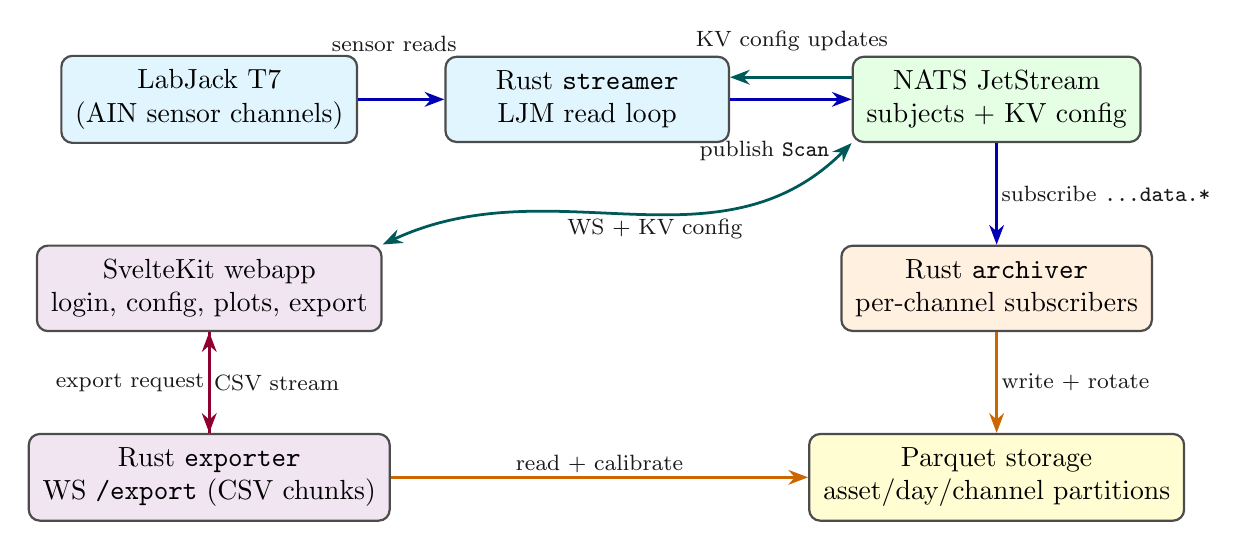
\begin{tikzpicture}[
  x=1cm,
  y=1cm,
  box/.style={
    draw=black!70,
    rounded corners,
    align=center,
    minimum width=3.6cm,
    minimum height=1.05cm,
    inner sep=5pt,
    line width=0.8pt
  },
  lbl/.style={font=\footnotesize, align=center, inner sep=1.3pt, text=black!90},
  data/.style={->, line width=1.0pt, draw=blue!70!black},
  cfg/.style={->, line width=1.0pt, draw=teal!70!black},
  storage/.style={->, line width=1.0pt, draw=orange!80!black},
  exportflow/.style={->, line width=1.0pt, draw=purple!75!black},
  >={Stealth[length=2.5mm]}
]
\node[box, fill=cyan!12] (labjack)  at (0.0,4.0)  {LabJack T7\\(AIN sensor channels)};
\node[box, fill=cyan!12] (streamer) at (4.8,4.0)  {Rust \texttt{streamer}\\LJM read loop};
\node[box, fill=green!10] (nats)    at (10.0,4.0)  {NATS JetStream\\subjects + KV config};

\node[box, fill=violet!10] (webapp)   at (0.0,1.6)  {SvelteKit webapp\\login, config, plots, export};
\node[box, fill=orange!12] (archiver) at (10.0,1.6)  {Rust \texttt{archiver}\\per-channel subscribers};

\node[box, fill=violet!10] (exporter) at (0.0,-0.8) {Rust \texttt{exporter}\\WS \texttt{/export} (CSV chunks)};
\node[box, fill=yellow!18] (parquet)  at (10.0,-0.8) {Parquet storage\\asset/day/channel partitions};

\draw[data] (labjack) -- (streamer);
\node[lbl] at (2.35,4.70) {sensor reads};
\draw[data] (streamer) -- (nats);
\node[lbl] at (7.05,3.34) {publish \texttt{Scan}};
\draw[cfg] ([yshift=8pt]nats.west) -- ([yshift=8pt]streamer.east);
\node[lbl, fill=white] at (7.40,4.74) {KV config updates};

\draw[data] (nats) -- node[lbl, right] {subscribe \texttt{...data.*}} (archiver);
\draw[cfg, <->] (webapp.north east) to[out=25,in=225] node[lbl, below, pos=0.55] {WS + KV config} (nats.south west);

\draw[exportflow] (webapp) -- node[lbl, left] {export request} (exporter);
\draw[exportflow] (exporter) -- node[lbl, right] {CSV stream} (webapp);

\draw[storage] (archiver) -- node[lbl, right] {write + rotate} (parquet);
\draw[storage] (exporter) -- node[lbl, above] {read + calibrate} (parquet);
\end{tikzpicture}

\end{document}
